\documentclass[11pt,letterpaper]{article}
\usepackage[utf8x]{inputenc}
\usepackage[T1]{fontenc}
\usepackage{amsmath}
\usepackage{amssymb}
\usepackage{graphicx}
\graphicspath{{../img/}}
\usepackage[spanish]{babel}

\title{Simulación Estocástica - Taller 1}
\author{Jesid Mauricio Mejía Castro}

\begin{document}
	\maketitle
	\section{Eventos y probabilidad}
	\begin{itemize}
		\item[a.] Supongamos que $A$ representa la canica azul; $R$, la roja y $V$, la verde. Entonces, dado que hay reemplazo, el espacio muestral para el experimento	de sacar una canica y después la siguiente es:
		\[
		\Omega = \{(A, A), (A, R), (A, V), (R, A), (R, R), (R, V), (V, A), (V, R), (V,
			V)\}.
		\]
		Si cada canica tiene la misma posibilidad de ser seleccionada, entonces la
		probabilidad de cada punto en el espacio muestral es $1/9$.
		\item[b.] Si se realiza el mismo experimento sin reemplazo, el espacio muestral sería:
		\[
		\Omega = \{(A, R), (A, V), (R, A), (R, V), (V, A), (V, R)\}.
		\]
		Es decir, se descarta la posibilidad de volver a sacar la misma canica.
	\end{itemize}
	
	\section{Valor esperado y varianza de una variable aleatoria discreta}
	Si $\Omega$ es el espacio muestral para el experimento de lanzar dos dados justos, se tiene que $|\Omega| = 36$. A continuación se muestra el espacio muestral. La función de masa de probablidad $p_M$ puede definirse con la auda de la siguiente tabla:
	
	\begin{center}
		\begin{tabular}{ | c | c c c c c c | c |} \hline
			$x$ & \multicolumn{6}{c}{$\Omega$} & $p_M(x)$ \\ \hline
			$1$ & $(1, 1)$ & $(1, 2)$ & $(1, 3)$ & $(1, 4)$ & $(1, 5)$ & $(1, 6)$ & $11/36$ \\
			$2$ & $(2, 1)$ & $(2, 2)$ & $(2, 3)$ & $(2, 4)$ & $(2, 5)$ & $(2, 6)$ & $9/36$ \\
			$3$ & $(3, 1)$ & $(3, 2)$ & $(3, 3)$ & $(3, 4)$ & $(3, 5)$ & $(3, 6)$ & $7/36$ \\
			$4$ & $(4, 1)$ & $(4, 2)$ & $(4, 3)$ & $(4, 4)$ & $(4, 5)$ & $(4, 6)$ & $5/36$ \\
			$5$ & $(5, 1)$ & $(5, 2)$ & $(5, 3)$ & $(5, 4)$ & $(5, 5)$ & $(5, 6)$ & $3/36$ \\
			$6$ & $(6, 1)$ & $(6, 2)$ & $(6, 3)$ & $(6, 4)$ & $(6, 5)$ & $(6, 6)$  & $1/36$ \\ \hline
			&  &  &  &  &  &  & $\sum_{x=1}^{6} p_M(x)=1$ \\ \hline
		\end{tabular}
	\end{center}
	
	A partir de la tabla podemos observar que 
	\[
	P(M \geq 3) = 1 - P(M < 3) = \frac{11}{36} + \frac{9}{36} = 0.\bar{5}.
	\]
	
	Para obtener el valor esperado, calculamos
	\[
	E(X) = \mu = \sum_{x = 1}^{6} x\,p_M(x) \approx 2.527.
	\]
	
	Para obtener la varianza, calculamos
	\[
	V(X) = \sigma^2 = \frac{1}{N} \sum_{x = 1}^{6} (x_i - \mu)^2 \approx 0.644.
	\]
	
	\section{Generadores congruentes}
	Los generadores de números aleatorios dados por la congruencia:
	\[
	X_{n+1} = (8X_n + 3) \mod 11
	\]
	generan los siguientes 11 ciclos variando la semilla $X_0$:

	\begin{verbatim}
		[x0=0]   3  5 10  6  7  4  2  8  1  0
		[x0=1]   0  3  5 10  6  7  4  2  8  1
		[x0=2]   8  1  0  3  5 10  6  7  4  2
		[x0=3]   5 10  6  7  4  2  8  1  0  3
		[x0=4]   2  8  1  0  3  5 10  6  7  4
		[x0=5]  10  6  7  4  2  8  1  0  3  5
		[x0=6]   7  4  2  8  1  0  3  5 10  6
		[x0=7]   4  2  8  1  0  3  5 10  6  7
		[x0=8]   1  0  3  5 10  6  7  4  2  8
		[x0=9]   9  9  9  9  9  9  9  9  9  9
		[x0=10]  6  7  4  2  8  1  0  3  5 10.
	\end{verbatim}
	
	\section{Método de la inversa para variables aleatorias discretas}
	\begin{itemize}
		\item[a.] La función de distribución acumulada (CDF) para X es:
		
		\[
		F_X(x) = 
		\begin{cases}
			0, &\quad\text{si}\quad x < 1 \\
			0.1, &\quad\text{si}\quad 1 \leq x < 1\\
			0.4, &\quad\text{si}\quad 2 \leq x < 5\\
			1, &\quad\text{si}\quad 5 \leq x.
		\end{cases}
		\]
		
		Su gráfica es la siguiente:
		
		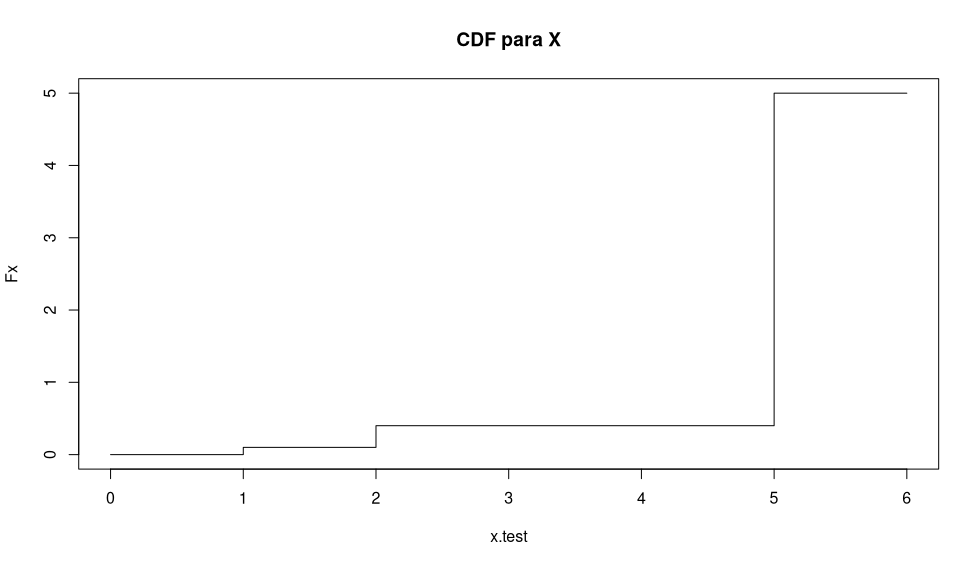
\includegraphics[height=6cm]{p4.png}
		
		\item[b.] Consultar el archivo \texttt{p4.R} adjunto.
		
		Para $n=10^3$ se obtiene la siguiente gráfica:
		
		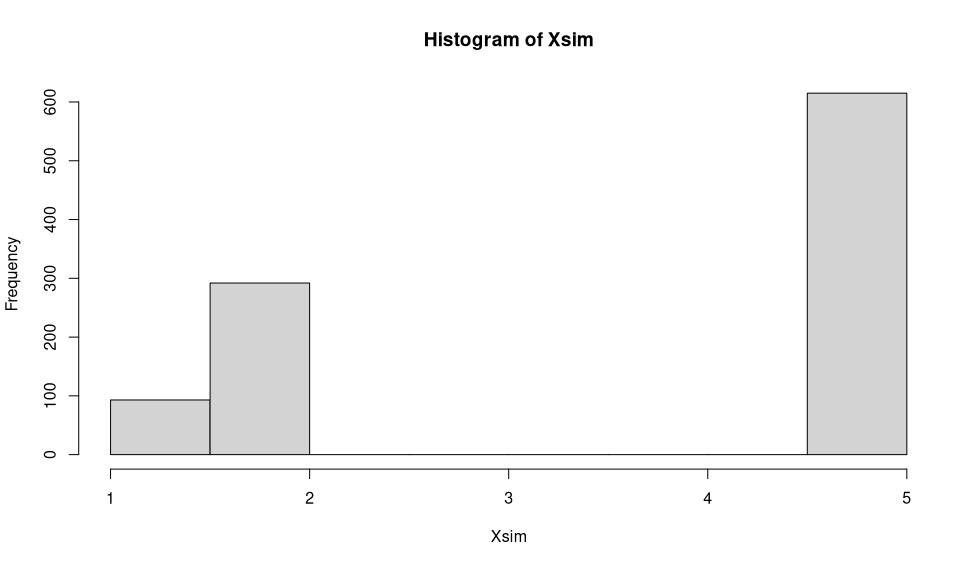
\includegraphics[height=6cm]{hist_10_3.png}
		
		Para $n=10^5$ se obtiene la siguiente gráfica:
		
		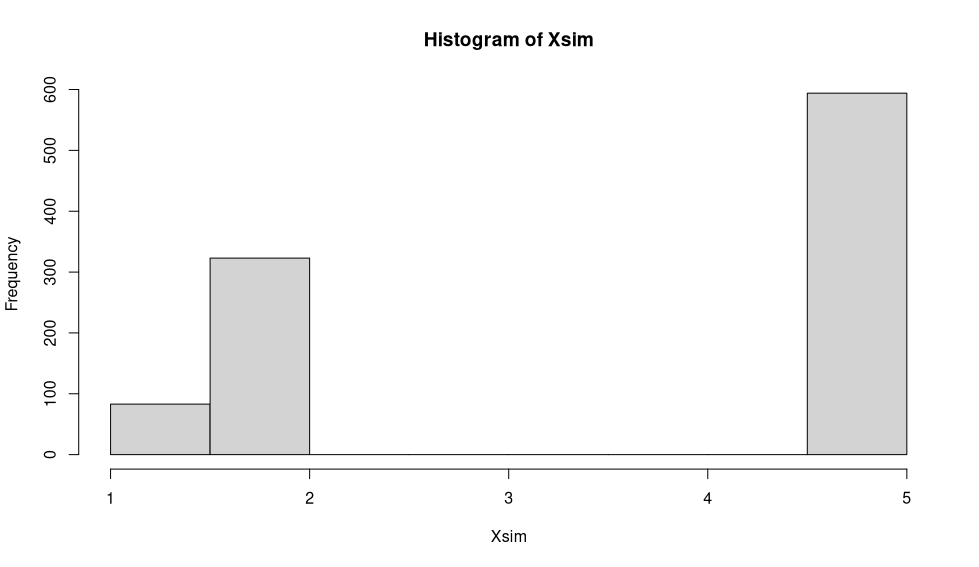
\includegraphics[height=6cm]{hist_10_5.png}
		
	\end{itemize}

	\section{Método de la inversa y método de rechazo para variable aleatoria contínua}
	
	Se nos da una variable aleatoria cuya función de densidad de probabilidad es:
	
	\[
	f_X(x) = 
	\begin{cases}
		3(x-1)^2 &\quad\text{si}\quad 1 < x \leq 2, \\
		0        &\quad\text{en otro caso.}
	\end{cases}
	\]
	
	\begin{itemize}
		\item[a.] Cálculo de probabilidades:
		
		\[ 
		P(X \leq 1) 
		= \int_{-\infty}^{1} f_X(x)\, dx = 0
		\]
		
		\[ 
		P(1 \leq X \leq 1.5) 
		= \int_{1}^{1.5} f_X(x)\, dx = 0.125
		\]
		
		\[ 
		P(1.5 \leq X) 
		= \int_{1.5}^{+\infty} f_X(x)\, dx 
		= \int_{1.5}^{2} 3(x-1)^2\, dx = 0.875.
		\]
		
		\item[b.] La función de distribución acumulada (CDF) $F_X(x)$ se obtiene calculando:
		
		\[ 
		F_X(x) = \int_{-\infty}^{x} f_X(u)\, du 
		= \int_{1}^{x} 3(u-1)^2\, du 
		= (x-1)^3\text{.} 
		\]
		
		\item[c.] Para simular núemeros aleatorios utilizando el método de inversión, debemos calcular $F_X^{-1}$ así:
		
		\[ 
		F_X^{-1}(x) = \sqrt[3]{\frac{x}{3}}-1 .
		\]
		
		Posteriormente, generamos un número aleatorio con distribución uniforme entre 0 y 1. Este número será el argumento de $F_X^{-1}$.
		
		\item[d.] Consultar \texttt{p5.R}.
		\item[e.] El histograma generado por el simulador es el siguiente:
		
		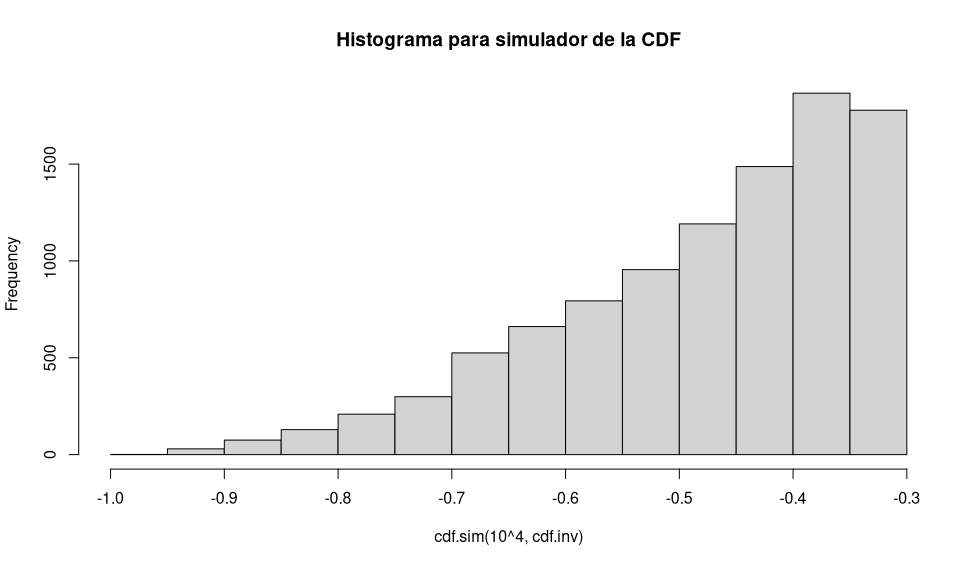
\includegraphics[height=6cm]{hist_p5_inv.png}
	\end{itemize}

	\section{Estimación de $\pi$}
	Sean $X$ y $Y$ variables aleatorios \emph{i.i.d.} $U(0,1)$.
	
	\begin{itemize}
		\item[a.] 
		
		\[
		P((X,Y) \in [a,b]\times[c,d]) = (b-c)(d-c).
		\]
		
		\item[b.] Basado en la respuesta anterior, si $A$ es subconjunto arbitrario del conjunto $[0,1]\times[0,1]$ La probabilidad $P((X,Y) \in A)$ puede interpretarse geométricamente como el área de la región $A$.
		
		\[
		P((X,Y) \in A) = \iint_A dA
		\]
		
		\item[c.] Si $A = \{(x,y)  \in [0,1]\times[0,1]: x^2 + y^2 \leq 1 \}$, entonces $A$ es un cuarto de circulo de radio 1 inscrito en el primer cuadrante. El área de $A$ es por tanto $\frac{\pi}{4}$.
		
		\item[d.] Consultar programa \texttt{p6.R}
	\end{itemize}

	\section{Integración de Monte Carlo}
	
	\begin{itemize}
		\item[a.] La integral
		
		\[
		\int_{-2}^{2} x^2 \, dx = \frac{16}{3} \approx 5.3
		\]
		
		Para la aproximación utilizando el método de Monte Carlo, consulte le programa \texttt{p7.R}
		
		\item[b] La integral
		
		\[
		\int_{0}^{1}\int_{0}^{2} e^{(x+y)^2} \, dx\,dy  \approx 275.884
		\]
		
		Para la aproximación utilizando el método de Monte Carlo, consulte le programa \texttt{p7.R}
		
	\end{itemize}
	
\end{document}
